\documentclass[a4paper]{article}
\usepackage[left=3cm, right=3cm]{geometry}
\usepackage[utf8x]{inputenc}
\usepackage{hyperref}
\usepackage{cite}
\usepackage{amssymb}
\usepackage{url}
\usepackage{float}
\usepackage{longtable}
\usepackage{array}
\usepackage{algorithmic}
\usepackage[boxed]{algorithm}
\usepackage{color}
\usepackage{graphicx}
\usepackage{tabularx}
\usepackage{caption,subcaption}
\pagestyle{headings}
\newcommand{\secondo}{\textsc{Secondo}}
\newcommand{\bmodb} {BerlinMOD Benchmark}
\newcommand{\op}[1]{\textbf{#1}}
\newcommand{\dt}[1]{\textsl{\underline{#1}}}
\newcommand{\true}{\textsl{TRUE}}
\newcommand{\false}{\textsl{FALSE}}
\newcommand{\secver}{2.9.x}
%opening
\title{Network Data Model and BerlinMOD Benchmark}
\author{Simone Jandt}
\date{Last Update: \today}
\begin{document}
\maketitle
\begin{abstract}
In the past, several data models for the representation of histories of
spatio-temporal data objects have been developed. We can categorize these data models
into data models for objects moving freely in the two dimensional space and data
models for network constrained moving objects. In this paper we select two representatives,
one for each data model category, which are both implemented in the \secondo{} DBMS,
and compare their capabilities with the \bmodb{}. We describe our implementation
of the used network constrained data model, and the translation
from the \bmodb{} into the network constrained data model and show
that in our experiments the network constrained data model outperforms the data
model of free movement in the two dimensional space by orders of magnitude.
\end{abstract}
\section{Introduction}
In the past, several data models for the representation of
spatio-temporal data objects have been developed. We can categorize them into
data models for objects moving freely in two dimensional space and data models
for network constrained objects. For both categories several diffferent data models
have been presented like
\cite{DataModelDataStructureGueting,RepresentingMovingObjectsGueting,STAUPelekis,HERMESMDCPelekis}
for spatio-temporal data objects moving freely in two dimensional space (DMFS) and
\cite{DynamicTransportNetworkDing,NetworkGueting,NetworkJensen,NetworkVazirgiannis}
for spatio-temporal data objects that are constrained by given networks (NCDM),
to name just a few. Objects which are restricted to use existing networks,
like cars are restricted to use road networks, can be represented as moving point
objects in both data models, whereas objects, which are not restricted by a given
network, like people, can be represented as moving point objects only in DMFS.

Why do we spend time on NCDM,if everything can be represented by
a DMFS? Now, it is natural to give positions related to the street
network instead of x,y-coordinates. NCDM are expected to use less storage space,
because geographical informations about street curves are stored only once in
the network, whereas in DMFS each street curve is stored in each moving point
object using this street. NCDM can support query processing with spezialized indexes,
because of the knowledge of the underlying network. And it is much easier to
formulate queries about the relationships between moving objects and the network
in the NCDM. And last but not least the results of our experiments show that
our network data model outperforms our data model of free movement in two dimensional
space by orders of magnitude. The network constrained data model uses less than
60\% of the storage space and less than 50\% of the total query run time of the
data model of free movement in space we used in our experiments.
We think that these results show that it is useful
to develop specialised data models for specialized data structures like NCDM for
newtork constrained moving objects to save storage space and reduce query run times.

For our benchmark experiments, presented in this paper, we chosed two data models
one for each data model category. Both data models use the same temporal representation
and are available in \secondo{} DBMS
\cite{SecondoEnvironmentDieker,SecondoPlatformPrototypingGueting}.
So we can exclude that different DBMS or temporal
representation issues bias the results of our data model comparison with the
\bmodb{}\cite{BerlinMODVLDBDuentgen}.
The DMFS we use is the data model presented in
\cite{RepresentingMovingObjectsGueting,DataModelDataStructureGueting}
(SPACE for short).
And the NCDM we use is the data model presented in \cite{NetworkGueting} (NET for short).
Our implementation of NET is described first in this paper (Section \ref{sec:implNDM}
and provides some further concepts which were only sketched in \cite{NetworkGueting}.

We used the \bmodb{} \cite{BerlinMODVLDBDuentgen} to compare the capabilities of
the two data models, because the \bmodb{} is to the best of our knowledge the
first benchmark for complete spatio-temporal database systems.
It is developed and available in \secondo{} DBMS. And the data generated by the
\bmodb{} data generator are restricted to the streets of the German capital Berlin,
such that they can be translated into a network constrained environment.
And last but not least, the data model used in the \bmodb{} is SPACE that we use
for our comparison. So we only have to translate the spatial and spatio-temporal
data types of the \bmodb{} once into our NET representation. This simplifies the
control of the query results and avoids errors caused by translation.
The translation of the spatial and spatio-temporal data types of the \bmodb{} data
into the NET representation described in this paper \ref{sec:Translation} can be
seen as an example for the usage of the \bmodb{} with other compatible data
representations or DBMS.

The rest of the paper is organised as follows: Related Work is presented in Section
\ref{sec:relWork}, including short reviews of the underlying \secondo{} DBMS
(Section \ref{sec:secondo}), the two data models (SPACE Section \ref{sec:bmodbdatamod}
and NET Section \ref{sec:netdatamod}) we chosed for our comparison, and the
\bmodb{} (Section \ref{sec:bmodb}).
In Section \ref{sec:implNDM} we give some informations about our implementation
of NET, the used operations and indexes.
The translation of the \bmodb{} data and query set into the NET representation
is described in Section \ref{sec:Translation}. The resulting experimental benchmark
setup is described in Section \ref{sec:scenario} followed by the results of our
experiments in Section \ref{sec:results}. We conclude our work in Section \ref{sec:summary}.
\section{Related Work}
\label{sec:relWork}
In the past many different spatio-temporal data models have been presented. Many
of them support only discrete spatio-temporal changes
\cite{sqlstchen,HunterWilliamson,Langran2,Langran1,Ramadrachan}
or deal only with current and future positions of continuously moving objects
\cite{MOSTWolfson}. Reviews of several different spatio-temporal data models are
given in \cite{ReviewSTDMPelekis}. In this paper we will focus on spatio-temporal
data models for complete histories of continuously moving objects. These can be
categorized into data models for objects moving freely in two dimensional space
(DMFS) and data models for network constrained moving objects (NCDM).

We will start with a few DMFS. \cite{MOLRaQSu} proposes the basic ideas of an
DMFS based on differential geometry and the linear constraints approach of modeling
spatial and spatio-temporal data. Spatial and spatio-temporal objects
are defined by linear constraints, and the queries use formulas from differential
geometry. The paper proposes only an incomplete abstract model without any usability.

\cite{STAUPelekis} and \cite{RepresentingMovingObjectsGueting,DataModelDataStructureGueting}
use both the idea of time sliced representation of moving objects first presented
in \cite{RepresentingMovingObjectsGueting}. \cite{DataModelDataStructureGueting}
supports only linear interpolation of movement, whereas \cite{STAUPelekis} also
supports arc interpolation. \cite{STAUPelekis} uses only one spatial
object containing all spatial geometries and one moving object for the
representation of the different moving object data types, whereas
\cite{RepresentingMovingObjectsGueting,DataModelDataStructureGueting} uses different
spatial and moving objects for the representation of the different
data types. Therefore \cite{STAUPelekis} provides only a single operator that
distinguishes between the different topological relationships via a parameter,
whereas \cite{RepresentingMovingObjectsGueting,DataModelDataStructureGueting}
uses different operations to estimate topological relationships. Alltogether
\cite{STAUPelekis} offers a more flexible object oriented design than
\cite{RepresentingMovingObjectsGueting,DataModelDataStructureGueting}.

The spatio-temporal framework proposed by
\cite{DataModelDataStructureGueting,RepresentingMovingObjectsGueting} is extended
by \cite{NetworkGueting} to be also usable in network constrained environments.
Similar to the most other NCDM in this section \cite{NetworkGueting} depends on
a fixed network representation. That means that the old network informations are lost when a
update of the network data structure occurs. Only \cite{DynamicTransportNetworkDing}
can handle such updates without loss of information.

\cite{NetworkVazirgiannis} proposes an edge based NCDM. With an relation holding
the edges and their attributes. The edge relation represents a undirected graph.
Moving objects are assumed to drive always on the path with the lowest cost
(distance or travel-time) from the source to the target point from a given
starting time. The trajectory is computed by this assumptation using the length
and speed attributes of the graph edges within the shortest / fastest path computation.
These assumptions will not always hold in real world environments. Such that the
moving object representation does not suffice real world requirements.

\cite{NetworkJensen} uses also an edge based network representation. The paper
proposes a combination of an 2D geometrical edge representation with an directed
graph representation of the network. Where as the 2D geometrical representation
handles the spatial information the connectivity information is mostly embedded
in the directed graph representation. The both representations are connected by
transition policies. Moving objects are represented by sets of 5 tuples. Each
5 tuple contains an edge identifier, the position of moving point on the edge
in terms of weight and length, the speed and direction of the movement, and
the time instant of this information.

Different from all other NCDM in this section \cite{DynamicTransportNetworkDing}
proposes a dynamic transportation network model. This means that the attributes
of the network parts are modelled by time depending dynamic attributes, such that
changes in the network environment can be handled without loss of information.
Similar to \cite{NetworkGueting} the idea of the network model bases
on routes and junctions. The authors propose a two-layer network representation
data structure, which combines the advantages of dynamic edge based
\cite{DynNetworkModEdgeGueting} and route based \cite{DynNetworkModRouteGueting}
NCDM approach. The route based environment reduces the update intervals and
used storage space for moving objects, whereas the edge-based envirionment supports
a more detailed view on the traffic conditions of the different edges belonging
to the same route. Moving objects are represented by a set of pairs of
motion vectors together with a boolean flag telling if the motion vector contains
actual or historical information. Each motion vector consists, in parts
similar to \cite{NetworkJensen}, of a time stamp, a network position, and a speed vector.

To the best of our knowledge only a few of these data models have been completely
implemented into different database management systems:
\begin{enumerate}
  \item \cite{STAUPelekis} is implemented as data cartridge \cite{HERMESMDCPelekis,
HERMESPelekis} for the commercial Oracle\textregistered ORDBMS \cite{ORACLE}.
  \item \cite{DynamicTransportNetworkDing} is implemented as extension of the
open source database project PostgreSQL \cite{PostgreSQL}.
  \item \cite{RepresentingMovingObjectsGueting,DataModelDataStructureGueting}
and \cite{NetworkGueting} are implemented in the freely available extensible
\secondo{} DBMS \cite{SecondoPlatformPrototypingGueting}.
\end{enumerate}

Although \cite{STAUPelekis} for the DMFS and \cite{DynamicTransportNetworkDing} for
the NCDM provide greater flexibility we decided to use
\cite{RepresentingMovingObjectsGueting,DataModelDataStructureGueting}
and \cite{NetworkGueting} in our experiments, because both are available in the
freely available \secondo{} DBMS. And not at least \secondo{} is the DBMS with
which the \bmodb{} \cite{BerlinMODVLDBDuentgen} was developed.

Other benchmarks for spatio-temporal databases provide only well defined
query sets \cite{QueriesTheordoridis} and a database description without data.
Or they come with well defined data generation, workload sets and experiments but
only to evaluate the capabilities of indexes for current and near future positions
\cite{COSTBenchmarkJensen}. Or they focus on time-evolving regional data and associated
index methods like \cite{BenchmarkTzouramanis}.

The \bmodb{} is to the best of our knowledge the only benchmark testing the capabilities
of complete spatio-temporal database systems. Coming with well defined data and
query sets feasible for moving objects in space and network constrained moving objects.

In the next sequel we give short reviews of the \secondo{} database system
(Section \ref{sec:secondo}), the both data models (Section \ref{sec:bmodbdatamod},
Section \ref{sec:netdatamod}) we used in our experiments, and the \bmodb{}
(Section \ref{sec:bmodb}).
\subsection{\secondo{} DBMS}
\label{sec:secondo}
The extensible \secondo{} DBMS presented in
\cite{SecondoEnvironmentDieker,SecondoPlatformPrototypingGueting} provides a
platform for implementing various kinds of data models. It provides a clean
interface between the data model independent system frame and the content of the
single data models. Hence \secondo{} can be easily extended by the user
implementing algebra modules to introduce new data types and operations on
these data types. The user may define additional viewers for the graphical user
interface or write additional optimization rules or cost functions to extend the
the optimizer. Since \secondo{} version 2.9 the users may publish their extensions
as a \secondo{} plugin such that other users can use these plugins to extend their own
\secondo{} system. They may use the newly provided functionalities or repeat the
published experiments. \secondo{} is freely available on the web \cite{secondoweb}.
It comes with a number of already implemented spatial and spatio-temporal data types
and operations including the DMFS (Section \ref{sec:bmodbdatamod}) and the NCDM
(Section \ref{sec:netdatamod}) used in this paper. Furthermore, the \bmodb{}
described in Section \ref{sec:bmodb} has been developed in the \secondo{} DBMS.
For our experiments we used the \secondo{} version \secver{}.
\subsection{Data Model of Free Movement in Two Dimensional Space}
\label{sec:bmodbdatamod}
\cite{STDTModelingQueryingMOinDErwig} presents the basic idea of the new
spatio-temporal data model that we will use as DMFS in our experiments. Besides
the general idea it discusses related work and the advantages of having abstract
and discrete data models. Abstract data models allow us to make definitions
in terms of infinite sets, without worrying whether finite representations exist.
They are useful as conceptual model, but they cannot be implemented, because computers
can only use finite sets. Data structures and algorithms have to work with finite
representations of the data types. Therefore we also need a discrete algebra
representation. The abstract definition of our data model has been published in
\cite{RepresentingMovingObjectsGueting}, whereas an associated discrete data
model was presented in \cite{DataModelDataStructureGueting}.

The type system in \cite{RepresentingMovingObjectsGueting} is defined using the
techniques presented in \cite{SecondOrderSignatureGueting}. The basic idea of
\cite{RepresentingMovingObjectsGueting} is to define type constructors
that create new data types if they are applied to an data type of a given set of
basic data types.
Basic data types are the standard data types like integer, real, string and Boolean (BASE);
the spatial data types point, points, line, and region (SPATIAL);
and the temporal type instant (TIME).

The data types of BASE are defined as usual. The SPATIAL data types are defined
by different carrier sets in the abstract and the disrete level.

In the abstract data model the carrier set of a point is $\mathbb{R}^2 \cup \{ \perp \}$.
In the discret data model the carrier set of a point is $\{ real \times real \} \cup \{ \perp \}$,
whereas the two $real$ values are interpreted as x,y-coordinates of a point in the
two dimensional plane.

In the abstract data model line and region are subsets of the set of point that
fullfill several conditions. In the discret data model a \dt{line} is a linear
approximation of the curve of the line by a finite set of line segments in the plane.
Regions are represented by a set of segments representing a linear approximation
of the region borders by polygons in the discrete data model.


The two most important type constructors are $moving$ and $range$. $Moving$
maps each type $\alpha$ from BASE and SPATIAL into an time dependend spatio-temporal
moving data type $moving$($\alpha$) (TEMPORAL), whereas $range$ is applicable to
BASE and TEMPORAL type $\beta$ and produces range data types $range$($\beta$).



In the abstract data model a time instant is a point in time or undefined, whereas
the carrier set for instant is $\mathbb{R} \cup \{ \perp \}$.
In \secondo{} all these spatial data types and many standard data types can be
''lifted'' to become time dependent \dt{moving} values. For all data types \dt{$\alpha$}
the constructor \dt{moving} creates a new data type \dt{moving}(\dt{$\alpha$})
(short form \dt{m$\alpha$}).

A car may be represented by a \dt{moving}(\dt{point}), short \dt{mpoint}.
An \dt{mpoint} consists of a set of units called
\dt{unit}(\dt{point}) (short form \dt{upoint}). Each \dt{upoint} consists of a time
interval and two \dt{point} values. The first \dt{point} value represents the
position of the \dt{mpoint} at the start of the time interval and the second
\dt{point} value represents the position of the \dt{mpoint} at the end of the
time interval. It is assumed that the object represented by the \dt{mpoint}
moves on the straight line between these two points with constant speed within the
given time interval. The velocity of the object is given by the ratio from the
distance of the two points and the length of the time interval of the unit.
All units of an \dt{mpoint} must have disjoint time intervals, because a car
cannot be at two different positions at the same time.
The units are sorted by ascending time intervals.

This spatio-temporal data model of \dt{moving} allows us to compute the position
of an \dt{mpoint} at every time instant within its definition time.
We can also compute the time instant the point passed a
given position assuming the \dt{mpoint} ever passes this position. The position of a
\dt{point} at a given time instant is represented by an \dt{intime}(\dt{point})
(short form \dt{ipoint}). An \dt{ipoint} consists of a time instant and a \dt{point} value.

Some other data types of \secondo{} which are used in the \bmodb{} are shown in
Table \ref{tab:bmodbdatatypes}.
\begin{table}[H]
\begin{center}
\begin{scriptsize}
\begin{tabularx}{1.0\textwidth}{|l|X|}
\hline
\textbf{Data Type} & \textbf{Description} \\
\hline
\dt{bool} & Usual boolean data type\\
\hline
\dt{int} & Usual integer number\\
\hline
\dt{real} & Usual real number\\
\hline
\dt{instant} & A point in time\\
\hline
\dt{periods} & A set of disjoint and not connected time interval\\
\hline
\dt{mbool} & A time dependent boolean value, which is constant \true{} or \false{}
within each \dt{ubool} \\
\hline
\dt{mreal} & Time dependent real number. Each unit is defined by a function
of time representing the \dt{real} value at each time instant.\\
\hline
\end{tabularx}
\end{scriptsize}
\caption{Other Data Types of \bmodb{}}
\label{tab:bmodbdatatypes}
\end{center}
\end{table}
\subsection{Network Data Model(NET)}
\label{sec:netdatamod}
The central idea of the NDM presented in \cite{NetworkGueting} is that
every movement is constrained by a given network and every position can be described
relative to this network. The data type \dt{network} is the central
data type in the NDM. All other data types of the NDM
are related to a given \dt{network} object by the unique network identifier that
is part of each \dt{network} object.

The \dt{network} object contains all spatial information of the represented network.
The \dt{network} consists of three main relations ($routes$, $junctions$, and $sections$),
two arrays providing fast access to adjacent network sections,
and some B-Tree and R-Tree indexes to supporting faster access to the main relations.

The relation $routes$ of the \dt{network} contains the attributes of the
streets like $id$, $route curve$, $route length$, and two Boolean flags. The first
flag indicates if the route starts at the lexicographically smaller end point or not.
The second flag indicates if the lanes of the street are separated like on German
Highways or not.

The $junctions$ relation of the \dt{network} contains all attributes of the street
crossings like the two route identifiers of the first and second street meeting at the
crossing, the distance of the crossing from the start of the first respectively
second street, tuple identifiers of the both streets in the routes relation,
tuple identifiers of the sections connected by this junction in the sections relation,
and a connectivity code telling us which lanes of the two streets are connected
by the crossing.

The $sections$ relation of the \dt{network} object contains the
attributes of the street parts between two crossings or a crossing and
the end of the street. These are the route identifier of the street the section
belongs to, the tuple identifier of this street in the routes relation, the start
position and end position of the section on the street, the section curve, and
again two Boolean flags with the same meaning as in the routes relation.

Furthermore there are two arrays in the \dt{network} object providing a fast
access from each section to their adjacent sections with respect to the driving
direction. Two sections are adjacent if their lanes are connected by a junction.

We created four B-Tree indexes for the route identifier attributes in the $routes$,
$junctions$ and $sections$ relation, and an R-Tree index over the curve attribute
of the $routes$ relation to support faster execution of operations dealing with
the relations of the \dt{network} object.

The data type \dt{gpoint} represents single positions in a given network. Besides the
network identifier a \dt{gpoint} consists of a route identifier, a distance from
the start of the route to the position of the \dt{gpoint} and a $side$ value
({$up$, $down$, $none$) telling us if the position is reachable from the $up$
or the $down$ side of the route in case of separated lanes. For simple
streets or positions which are reachable from both sides of the route, the side
value is always $none$.

Parts of the network, regardless if they represent paths or regions, are given as
\dt{gline} values. Besides the network identifier, a \dt{gline} consists of a set
of \dt{RouteInterval}s, and two Boolean flags. The Boolean flags tell us if the
\dt{gline} is defined and if the set of \dt{RouteInterval}s is sorted.

Each \dt{RouteInterval} consists of a route identifier identifying the route that
the route interval belongs to, and the start and the end position of the
route interval on this route
\footnote{In the original paper the \dt{RouteInterval} includes a $side$ value
analogous to the \dt{gpoint}. But this parameter is not yet part of the implementation.}.
We call a \label{sec:sortedgline} set of \dt{RouteInterval}s sorted if the following
conditions are fullfilled:
\begin{itemize}
   \item all \dt{RouteInterval}s are disjoint
   \item the \dt{RouteInterval}s are stored in ascending order of their route identifiers
   \item if two disjoint \dt{RouteInterval}s have the same route identifier, the
\dt{RouteInterval} with the smaller start position is stored first
   \item for all \dt{RouteInterval}s, the $start$ $position \le end$ $position$
\end{itemize}
Many algorithms take profit from sorted \dt{gline} values. For example: If $n$
is the number of the route intervals in a \dt{gline}, the
decision, if a \dt{gpoint} is inside the \dt{gline} needs O($n$) time for unsorted
and O($\log n$) time for sorted \dt{gline} values.

Unfortunately not all \dt{gline} values can be stored sorted. If a \dt{gline}
value represents a path between two \dt{gpoint} in the network, we need the
route intervals exactly in the sequence they are used in the path. This will
nearly never be a sorted set like defined before.  We store \dt{gline}
values sorted whenever this is possible to support faster query execution, and
introduced a Boolean sorted flag. Every algorithm which deals with \dt{gline} values
checks this flag and uses the corresponding code.

Mostly similar to the \dt{mpoint} of the other data model there is an
\dt{mgpoint} in the NDM. An \dt{mgpoint} consists of a set of
\dt{ugpoint} with disjoint time intervals. Each \dt{ugpoint} consists of a time
interval and two \dt{gpoint} values. Every time the \dt{mgpoint} changes the route
or the speed, a new \dt{ugpoint} is written. Each \dt{ugpoint} is assumed to follow
the same route from the start to the end position at the same speed. So accordingly
to the \dt{mpoint} we can compute the network position of the \dt{mgpoint} at every
time instant within the definition time of the \dt{mgpoint} as \dt{intime}(\dt{gpoint}).

In deviation from the original NDM we extended the implementation
of the \dt{mgpoint} with four additional attributes to support faster query execution:
\begin{enumerate}
   \item The total driven distance
   \item A sorted set of \dt{RouteInterval}s representing the positions ever
traversed by the \dt{mgpoint}
   \item A Boolean defined flag for the set of \dt{RouteInterval}s
   \item A spatio-temporal minimum bounding box
\end{enumerate}
The sorted set of \dt{RouteInterval}s was introduced, because analogous to sorted
\dt{gline} values it makes it much faster to decide whether an \dt{mgpoint} ever passed
a given network position or not. Instead of a linear check of all $m$ \dt{ugpoint}s
of an \dt{mgpoint} we can perform a binary scan on the much smaller number $r$ of
the passed \dt{RouteInterval}s.
This reduces the time complexity from O($m$) to O($\log r$) for the \op{passes}
operation.

The spatio-temporal minimum bounding box was introduced as an parameter to the
\dt{mgpoint} because the computation of this value is very expensive in the
NDM. Although each unit of an \dt{mgpoint} stays on the same route
at the same speed it may follow different spatial directions. For example, a route may
lead uphill in serpentine. A spatial bounding box only computed from the spatial
start and end position may not enclose all spatial positions of the car within
the unit. Therefore we always have to examine the spatial dimensions of the
\dt{RouteInterval} passed within a unit to compute the units bounding box. This
needs an access to the route curve in the $routes$ relation of the corresponding
\dt{network} object. If $r$ is the number of routes
of the network and $h$ the number of \dt{HalfSegment}s belonging to the \dt{RouteInterval}
passed in a unit, we need O($h + \log r$) time to
compute the bounding box for a single unit. The bounding box of the \dt{mgpoint}
is the union of the bounding boxes of its $m$ units. So the computation of the
spatio-temporal respectively spatial bounding box of an \dt{mgpoint} needs
O($H + m \log r)$) time, with $H = \sum_{i=1}^m {h_i}$ if $h_i$ is the number of the
$half$ $segments$ for unit $i$, $1 \leq i \leq m$ of the \dt{mgpoint}. This very expensive computation is only done
on demand or if we can get the bounding box for free. For example we can copy
the bounding box of an \dt{mpoint} at the translation time into an \dt{mgpoint}
without big computational costs. The bounding box attribute is not maintained. If
the \dt{mgpoint} value changes, the bounding box attribute is set to be undefined
until recomputing is necessary.
\subsection{BerlinMOD Benchmark}
\label{sec:bmodb}
The \bmodb{} was presented in \cite{BerlinMODVLDB} and the
provided scripts for the data generator are implemented as \secondo{} DBMS operations.
The \bmodb{} is available on the web \cite{berlinmodweb} and provides a well defined
data-set and queries for the experimental evaluation of the capabilities of
spatial and spatio-temporal database systems dealing with histories of moving
objects. The \bmodb{} emphasises the development of complete systems
and simplifies experimental repeatability pointing out the capabilities and the
weaknesses of the benchmarked systems.

The data-sets of the \bmodb{} are created using the street map of the German
capital Berlin \cite{bbike} and statistical data about the regions of Berlin
\cite{bevberlin,berlinstadtatlas} as input relations.
The created moving objects represent cars driving in the streets of Berlin,
simulating the behaviour of people living and working in Berlin.
Every moving object has a home node and a work node. Every weekday each car will
do a trip from the home node to the work node in the morning and vice versa
in the late afternoon. Beside this, randomly chosen cars will make additional
trips in the evening and up to six times at the weekend to randomly chosen
targets in Berlin and back home. The \bmodb{} uses the data model of free movement in two
dimensional space described in Section \ref{sec:bmodbdatamod}. Because the \bmodb{}
generates all data sets restricted to the street map of Berlin, the \bmodb{} can
also be used for network constrained data models, if the spatial and spatio-temporal
data types are translated into a corresponding NDM, like we did
for our experiments.

The number of observed cars and the duration of the observation period can be
influenced by the user setting the $scalefactor$ to different values in the data
generation script of the \bmodb{}. For example at $scalefactor$ 1.0 the data generator
creates 2000 moving point objects observed for 28 days, each of them sending a
GPS-signal every 2 seconds. These simulated signals are simplified such that time
intervals when a car does not move or moves in the same direction at the same
speed are merged into one single time interval. For example: If a car is parked in front
of the work node for 8 hours, there will be only one entry in the history of the
cars movement with a time interval of 8 hours instead of 14.400 entries,
one for each GPS time interval.

The \bmodb{} provides two different approaches to store the histories of moving
objects, called the object-based approach (OBA) and the trip based approach (TBA),
respectively.

In the OBA, the complete history for each moving object is kept together in one
single entry. There is only one relation $dataScar$
containing one tuple for each object consisting of the spatio-temporal data of
the object $journey$, the $licence$, the $type$, and the $model$ of the object.

In the TBA, we have two relations $dataMcar$ and $dataMtrip$. $dataMcar$ contains
the static data for each object like $licence$, $type$, and $model$ together with
an object identifier $moid$. $dataMtrip$ contains for each $moid$ several tuples,
each of them containing all units of a single trip of the moving object, or a
single unit for a longer stop. For example, each time the car drives from home node
to work node is a single trip, and each time the car is parked in front of the office
is also a single trip.

Besides the moving point objects, the \bmodb{} provides several data sets, each of them
containing 100 pseudo randomly generated data objects, which are used in the
benchmark queries. Table \ref{tab:queryobjects} gives an overview of these query
objects. The \bmodb{} deals also with subsets from these query object sets consisting
of the first or second 10 query objects of a query object set. They are labeled
by the name of the query object set followed by a 1 for the first ten or a 2 for
the second ten query objects.

\begin{table}[H]
  \begin{tabularx}{1.0\textwidth}{|l|X|}
    \hline
    \textbf{Name of Data Set}&\textbf{Tuple Content}\\
    \hline
    $QueryPoints$&Object identifier and \dt{point} value\\
    \hline
    $QueryRegions$&Object identifier and \dt{region} value\\
    \hline
    $QueryInstants$&Object identifier and time instant\\
    \hline
    $QueryPeriods$&Object identifier and time interval\\
    \hline
    $QueryLicences$& Object identifier and a \dt{string} representing a licence value\\
    \hline
  \end{tabularx}
  \caption{Query Object Relations of \bmodb{}}
  \label{tab:queryobjects}
\end{table}

The \bmodb{} provides two sets of queries BerlinMOD/R and BerlinMOD/NN.
BerlinMOD/R addresses range queries and BerlinMOD/NN nearest neighbour queries.
In this paper we will focus on the range queries, which are the main aspect of the
\bmodb{} up to now.

The query set BerlinMOD/R includes 17 queries selected of the set of possible
combinations of the 5 aspects:
\begin{itemize}
  \item known or unknown object identity,
  \item standard attribute, spatial, temporal, or spatio-temporal dimension,
  \item point, range, or unbounded query interval,
  \item single object or object relationships condition type,
  \item with or without aggregation.
\end{itemize}
We will present the 17 queries in more detail in Section \ref{sec:queries}
together with our NDM algorithms for these queries.
\section{Implementation Issues}
\label{sec:implNDM}
\section{Translation of BerlinMOD into Network Data Model}
\label{sec:Translation}
In this section we describe the creation of the \dt{network} object from the $streets$
value of the \bmodb{} in Section \ref{sec:createNetwork}. In Section
\ref{sec:translateSTdata} we describe how to use this new created \dt{network}
value as a reference for the translation of all spatial and spatio-temporal data
type objects of the \bmodb{} into the NDM representation.
In Section \ref{sec:createIndex} we describe the indexes we build on the NDM
representation to support faster query execution. We close this part
with Section \ref{sec:queries} were we describe the executable \secondo{} queries
for the NDM representation of the \bmodb{}.

Executable \secondo{} scripts for the network and index creation, object translation,
and the network benchmark queries can be downloaded from our web site \cite{NetworkWeb}.
\subsection{Create Network Object}
\label{sec:createNetwork}
The \dt{network} object $net$ is created by extracting the $routes$ data from
the $streets$ object that is created by the BerlinMOD Data Generator.
The extracted data $r$ is used to compute the crossings of the
routes of Berlin $j$. The data source lacks information about the connectivity
of the street crossings, such that we use the maximum value for the connectivity
code of each crossing as default value in this step.
Now we can use $r$ and $j$ as input relations for the operator \op{thenetwork}
to create our \dt{network} object $net$ representing the streets of Berlin in
the NDM representation of the \bmodb{}.

The network creation algorithm first copies all tuples of $r$ to the
$routes$ relation of $net$ and creates the B-Tree index on the route
identifiers and the R-Tree index on the route curves of the $routes$ relation of
$net$. Then all tuples of $j$ are copied to the $junctions$ relation
of $net$ and the tuple identifiers for the both routes connected
by this junction are added to the junctions entry. After that we build two B-Trees
indexing the route identifiers of the first respectively second route in the
$junctions$ relation. Next for every route of the $routes$ relation all junctions
on this route are taken from the $junctions$ relation to compute the up and
down sections for each of this junctions on the route. The up and down
sections are inserted into the $sections$ relation of $net$ and the
tuple identifiers of the sections are added to the entry of the corresponding
junction in the $junctions$ relation. After that the B-Tree index for the
route identifiers in the $sections$ relation is created and the adjacency
lists of $net$ are filled with the adjacent section pairs defined by the
$junctions$ relation.

If $|r|$ is the number of routes and $|j|$ is the number of junctions,
the algorithm needs O($|r| \log |r|$) time to copy $r$ to the
$routes$ relation of $net$ and create the indexes of the
$routes$ relation. The creation of the $junctions$ relation and the build
of the B-Tree indexes takes O($|j| \log |j|$) time.
O($|r|J$)\footnote{$J = \sum_{i=1}^{|r|}{j_i}$, where $j_i$ is the number of
junction on route $i$, with $i \leq 1 \leq |r|$} time is needed to fill the
$sections$ relation and O($|j|$) time to fill the $adjacency lists$ of $net$.
Altogether the complete algorithm needs:
O($|r| \log |r|+|j| \log |j| + |r|J$) time to create the $net$ from the two input
relations $r$ and $j$.
\subsection{Translate Spatial and Spatio-Temporal Data Types}
\label{sec:translateSTdata}
In this section we describe the translation of the spatial and spatio-temporal
data types of the \bmodb{} data set into network respectively network-temporal
objects. All translations are done relative to the \dt{network} object $net$ that
we described in Section \ref{sec:createNetwork}.
All algorithms in this section get a spatial respectively spatio-temporal \bmodb{}
data type object and the \dt{network} object $net$ as input. They return the
corresponding NDM object respectively an undefined NDM object if the input data
object is not constrained by $net$.
\subsubsection{Translate \dt{point} into \dt{gpoint}}
The \op{point2gpoint} operation translates a \dt{point} value $p$ into a corresponding
\dt{gpoint} value $gp$ if possible. This operation is also included in the other translation
operations. The algorithm uses the R-Tree index of the
$routes$ relation of $net$ to select the route curve closest to $p$ and computes the
position of $p$ on this route curve. In case of the \bmodb{} the $side$ value of
$gp$ is always set to $none$, because the \bmodb{} does not differentiate between
the different sides of a street.

If $r$ is the number of routes in the $routes$ relation
and $k$ is the number of routes, which route curve bounding boxes contain p,
the worst case complexity of the algorithm is O($\log{r} + k$).

This should be all to translate the \dt{point} values of the $QueryPoints$
relation of the \bmodb{} into network query positions. But there is a problem with
the NDM representation of junctions. In the NDM, contrary to the DMFS, each junction
has more than one \dt{gpoint} representation, because each junction is related to
two or more routes. Hence if a junction position is given related to route $a$
we won't detect the junction as passed if an \dt{mgpoint} object passes the junction
on route $b$ in all cases, because the definition of \op{passes} in the network
data model is slightly different from the \op{passes} operation in the \bmodb{} data model.
Unfortunately all query points of the \bmodb{} are junctions. To make the results
comparable, we added an operator \op{polygpoints}, which returns for every input
\dt{gpoint} value $gp$ a stream of \dt{gpoint} values. If $gp$ represents a junction
we return all \dt{gpoint} values representing the same junction in $net$,
otherwise we return only $gp$ in the stream. So we got 221 query \dt{gpoint}
values in $QueryPointsNet$ for the 100 query \dt{point} values in
$QueryPoints$ and 22 \dt{gpoint} values in $QueryPoints1Net$ for the
10 \dt{point} values of $QueryPoints1$ of the \bmodb{}. This means we always have
to compute the results for the double number of query points in our NDM relativ
to the DMFS.
\subsubsection{Translate \dt{mpoint} into \dt{mgpoint}}
The second operation \op{mpoint2mgpoint} translates an \dt{mpoint} value $s$
into an \dt{mgpoint} value $t$. The main idea of the algorithm is to use the
continuous movement of $s$ to reduce computation time. We initialize the
algorithm by reading the first unit of $s$ and use the \op{point2gpoint}
algorithm to find a route in the network containing the $start$ and
the $end point$ of this unit. We initialize the first unit of $t$ with
the computed network values. Then we read the next unit of $s$ and try to find
the $end point$ of the new unit on the same route the last unit of $s$ was
found. If the $end point$ is found on the same route we check the moving direction
on the route and speed of the point in the unit. If they are equal to the actual unit we extend
the actual unit of $t$ to enclose the value of the actual unit of $s$. If the
speed or the moving direction on the route changes we write the actual unit to $t$ and initialize
a new unit for $t$ with the network values of the actual unit from $s$.
If the $end point$ can't be found on the same route as the last unit from
$s$, we write the actual unit of $t$ and start a search on the route curves
of the adjacent sections to find the route curve that contains the $start$
and the $end point$ of the actual unit of $s$. We initialize a new unit
for $t$ with the estimated network values for the actual unit of $s$ and
continue with the next unit of $s$. At last we add the actual network unit
to $t$.

The time complexity to find the start values for the first unit is the time complexity
from \op{point2gpoint} O($\log r + k$).
For each of the next $m$ units of $s$, the time complexity is O(1) if $s$ does not
change the route. And it is O($a$) if the end point is on another route and $a$ is the maximum
number of adjacent sections. So we get a worst case time complexity of
O($\log r + k + ma$) for the translation of an \dt{mpoint} $s$ into an \dt{mgpoint} $t$.
\subsubsection{Translate \dt{region} into \dt{gline}}
The translation of the \dt{region} values in the $QueryRegions$ relation of the
\bmodb{} into \dt{gline} values of our NDM is done in several steps.
First of all we build a single big \dt{line} object containing all network streets.
Then we compute for each \dt{region} of the $QueryRegions$ the intersection with
this big \dt{line} object. At last we translate the resulting \dt{line} objects
of the intersection, each representing one \dt{region} of the $QueryRegions$
relation, into sorted \dt{gline} values using the \op{line2gline} operation.

The algorithm of the \op{line2gline} operation takes each \dt{HalfSegment} of a
\dt{line} value and computes a corresponding network \dt{RouteInterval} by
searching a common $route curve$ for the $start$ and the $end point$ of the
\dt{HalfSegment} using the \op{point2gpoint} operation. The computed
\dt{RouteInterval}s are sorted, merged and compressed before the resulting
\dt{gline} value is returned. If the number of \dt{HalfSegment}s of a \dt{line}
value is $h$ and the number of resulting compressed \dt{RouteInterval}s is $r$
we get a time complexity of O($h$O(\op{point2gpoint})$+ h \log r + r$) for the
whole algorithm. Whereby the summand $h \log r + r$ is caused by the compressing
and sorting of the resulting \dt{gline} but as mentioned before
in \ref{sec:sortedgline} we think this time is well invested, because it is needed
once and the sorted \dt{gline} value is used many times.
\subsection{Create Indexes on Network Data Model}
\label{sec:createIndex}
For the use with the \bmodb{} we created the following indexes on the network
data model representation of the \bmodb{} data sets:
\begin{itemize}
  \item B-Tree indexes for the $licences$ and $moid$ attributes of the relations
$dataSNcar$, $dataMcar$, and $dataMNtrip$. These indexes are similar to the indexes
created in the \bmodb{} for $dataSCcar$, $dataMCcar$, and $dataMCtrip$, because
the relations $dataSNcar$, $dataMcar$ and $dataMNtrip$ contain the network
data model representation of the $dataScar$, $dataMcar$ and $dataMtrip$ relation
of the \bmodb{}, respectively. We don't explain them in more detail.
  \item An R-Tree index of the spatio-temporal bounding boxes of the \dt{mgpoint}
attributes in the $dataMNtrip$ and the $dataSNcar$ relation. Different from the
data model that uses the spatio-temporal units for the spatio-temporal indexes, we
used only the big bounding boxes of the whole trips instead of the much smaller
bounding boxes for each single unit as it is done in the DMFS.
 \item For every unit of each \dt{mgpoint} we build a temporal-network bounding box
and for every \dt{RouteInterval} of every \dt{mgpoint}s trajectory a network bounding box.
These network bounding boxes ($netboxes$ for short) are used to create R-Trees
indexing the network and temporal-network positions of the \dt{mgpoint}s.
A temporal-network bounding box
is a degenerated three dimensional rectangle. The coordinates are defined to be
$x_1 = x_2 = route identifier$ as a \dt{real} value (The equality of $x_1$ and
$x_2$ makes the degeneration.), $y_1 = \min (start position, end position)$,
$y_2 = \max (start position, end position)$,
and, $z_1 = start time$ as a \dt{real} value and $z_2 = end time$ as a \dt{real} value.
The network bounding box is defined to be a degenerated two dimensional rectangle
with x,y-coordinates analogous to the temporal-network boxes.
\end{itemize}
\subsection{Translate Benchmark Queries}
\label{sec:queries}
We developed executable \secondo{} queries for each of the 17 BerlinMOD/R queries
for the OBA and the TBA using our network indexes to support faster query execution.
The \secondo{} optimizer is not able to optimize SQL-queries on NDM objects yet, so we tested in
our experiments many different query formulations for each query to get optimal
queries delivering the correct result in a minimum of time.

The limited space does not allow us to show all our executable \secondo{} queries
for the NDM in detail, but they can be downloaded as \secondo{} scripts
from our web page. Here we give only a short overview over the \bmodb{} queries
and their NDM algorithms.

Every time we need a licence in the result or have a query licence number we need
an additional step in the TBA, because we have to join the $dataMNtrip$ and $dataMcar$
relation using the $moid$ attribute and the corresponding B-Tree indexes.
We will not repeat this step at every single TBA query description.

Query 1 asks for the models of the cars with licence plate numbers from $QueryLicences$,
and query 2 for the number of vehicles that are ``passenger cars''. Both queries
deal only with standard attributes; so we only changed the relation names and the
B-Tree indexes to match the NDM representation.

Query 3 searches for the positions of the ten cars from $QueryLicence1$ at the
ten time instants from $QueryInstants1$. We use the licence B-Tree to select the
ten cars and compute the positions of these ten cars for each of the ten time
instants from $QueryInstants1$ if the time instant is inside the definition time
of the trip.

Query 4 asks for the licence numbers of the cars that passed the points
from $QueryPointsNet$. We create a $netbox$ for each \dt{gpoint} in $QueryPointNet$
and use our specialised $netbox$ R-Tree of the \dt{mgpoint} \dt{RouteInterval} to
select the vehicles passing the given query points.

The queries 5, 6, and 10 deal with Euclidean distance values, which are not very
useful in network environments. In networks everything is constrained by the
network and normaly the network distances are computed instead of Euclidean
distances. We decided to retranslate intermediate results
into spatial respectively spatio-temporal objects and use the existing
Euclidean distance operation to compute the distances between this objects to make
the results comparable.

Query 5 asks for the minimum distance between places where vehicles with
licences from $QueryLicence1$ and $QueryLicence2$ have been. We select the cars
with licence plate numbers from $QueryLicence1$ respectively $QueryLicences2$ using the
B-Tree over the $Licence$ attribute of the $dataSNcar$ relation. In the TBA, the
resulting trajectories for each car are aggregated into one single trajectory
for each car. In both approaches we create a \dt{line} value for each resulting
(aggregated) trajectory value of the \dt{mgpoint}s and compute the Euclidean distance
between these \dt{line} values for each pair of licences one from $QueryLicences1$ and one
from $QueryLicences2$.

Query 6 asks for the pairs of licences from ``trucks'' that have been as close as
10m or less to each other. We filter $dataSNcar$ relation, respectively $dataMcar$
relation to select the ``trucks'' and compute the spatio-temporal bounding box
of each trip of a ``truck''. We extend the spatial dimensions of the bounding boxes
by 5m in each spatial direction and retranslate the \dt{mgpoint} values into \dt{mpoint}
values in a first step. In a second step, we compute the join of the results from
step one with itself using the intersection of the bounding boxes as join criteria.
We filter the result to include all licence pairs of ``trucks'' that had sometimes
a distance lower than 10m. In the TBA, we additionally remove the duplicate licence
pairs from the result.

Query 7 asks for the licence plate numbers of the ``passenger'' cars that reached
the points from $QueryPoints$ first of all ``passenger'' cars during the
observation period. The first step to solve query 7 in the NDM is
equal to query 4. In a filter step we remove all ``not passenger'' cars from the
first intermediate result. We compute for each remaining candidate trip the times
the trip reaches first the query positions. We group the resulting time instants
by the identifiers of the query positions and compute the minimum time stamp of
each group, which is in fact the first time the query position was reached by a
car. In a last step the licences of the ``passenger'' cars reaching the query
positions at this first time instant are computed using the specialised
network-temporal index of the NDM.

Query 8 computes the overall travelled distances of the vehicles from $QueryLicence1$
within the periods from $QueryPeriods1$. We select the candidate cars using the
licence B-Tree, restrict the trips to the query periods and return the lengths of the
trips in the OBA. In the TBA we have to sum up the length of the different
trips driven by a single car within each query period.

Query 9 asks for the longest distance travelled by a single vehicle during each
of the periods from $QueryPeriods1$. We restrict all trips to the periods, compute
the driven distances and select the maximum length for each query periods value.
Again we have to do an additional aggregation of the distances driven from the same
car in the same period in the TBA.

Query 10 asks when and where vehicles with licences from $QueryLicence1$ meet which
other vehicles (distance less than 3m). In the OBA we first retranslate every
\dt{mgpoint} value of $dataSNCar$ into a \dt{mpoint} value and extend the spatial
bounding box of each of this trips by 1.5 m in every spatial direction. After that we
select the ten candidate trips given by $QueryLicences1$, retranslate them and
extend their spatial bounding boxes in the same way. We join all trips from the
first two steps where the extended bounding boxes intersect and filter the
candidate pairs that have different licences and their distance is sometimes
less than 3m to each other. We compute the position of the \dt{mgpoint} at the
times the distance between the remaining candidate pairs of \dt{mpoint} was less
than 3 m and return the licence pairs and the network positions of the first car
when it has been closer than 3 m to the other one.

In the TBA we select the trips given by $QueryLicences1$ from
$dataMNtrip$, retranslate them into \dt{mpoint} values, and extend their spatio-temporal
bounding boxes by 3m in each spatial direction. After that we use the spatio-temporal
index of $dataMNtrip$ to select for each trip of the ten cars, the cars
of $dataMNtrip$ which spatio-temporal bounding boxes intersect the extended spatio-temporal
bounding boxes built before. For every pair of candidate trips we
retranslate the second trip and use the Euclidean Distance function for \dt{mpoint}
values to determine the times when the both \dt{mgpoint} had a distance less than 3m.
At last we restrict the trip of the query \dt{mgpoint} to this times and
aggregate the resulting trips into one single trip for each licence pair.

In our experiments we tried out several indexes to support a faster query execution
of query 10 including the MON-Tree presented in \cite{MONTreeAlmeidaGeoinformatica}. The MON-Tree showed
very good CPU times but never the less the total run time was very high. In the end
the simple form described above showed the best complete run time performance of all
indexes.

Query 11 asks for the vehicles that passed a point from $QueryPoints1Net$ at one of the
time instants from $QueryInstants1$. We build a network-temporal query box from the
$QueryInstant1$ and $QueryPoints1Net$ relation and use the network-temporal index
on $dataSNcar$, respectively $dataMNtrip$, to select the resulting trips.

Query 12 asks for the vehicles that met at a point from $QueryPoints1Net$ at an time
instant from $QueryInstants1$. The first step of query 12 is identical with query 11.
In a second step the Cartesian Product of the result of the first step with itself
is computed and filtered for vehicles which have been at the same query point
at the same query time instant.

Query 13 asks for the vehicles which travelled within one of the regions from
$QueryRegions1Net$ during the periods from $QueryPeriods1$. We restrict the trips
to the query regions and check if the restricted trips are defined within the query
periods. In TBA possible duplicate licence pairs have to be removed and the
resulting $moid$s must be mapped to the licences of the cars to generate the result
using the B-Tree $moid$ index of $dataMcar$.

Query 14 asks for the vehicles that have been in one of the regions from $QueryRegions1Net$
at a time instant from $QueryInstants1$. We build temporal-netboxes from the query
objects to select candidate trips using the temporal-network position index. We refine the
result filtering the candidate trips really full filling the query predicates.

Query 15 asks for the vehicles passing a point from $QueryPoints1Net$ during a period
from $QueryPeriods1$. Analogous to query 14 we build temporal-netboxes of the
of the query parameters to select the candidate trips using the temporal-network
position index and refine the result filtering the candidates really fullfilling
the query constraints.

Query 16 asks for the licence pairs one from $QueryLicence1$ and one from $QueryLicence2$
of vehicles, which were both present in a region from $QueryRegions1Net$ within a period
from $QueryPeriods1$, but did not meet there and then. We select the candidate trips
using the licence B-Tree of $dataSNcar$ relation and restrict the resulting trips to be
\op{present} during the query periods and \op{inside} the query region. This is done
one time for the licences from $QueryLicences1$ and one time for the licences from
$QueryLicences2$. The both intermediate results are joined and filtered to get the
trips of different cars which where at the same period in the same region
without meeting each other there and then. In the TBA we have
to do a additional selection from trips with the $moids$ belonging to the cars
selected before by the licences and remove duplicates of licence pairs from the
same period and region.

Query 17 asks for the points from $QueryPointsNet$ that have been visited by a
maximum number of different vehicles. In a first step we use almost the query
algorithm from query 4 to select the trips passing a given query
point. After that we group the cars passing query points by the ids of the
query points and count the number of cars passing this query point. In a last
step the point(s) with the maximum number of passing cars is(are) selected.
In the TBA we have to remove duplicate vehicles from the result list before we
count the number of passing cars.
\section{Experimental Setup}
\label{sec:scenario}
For our experiments we used a standard personal computer with an AMD Phenom II X4
Quad Core 2.95 GHz CPU, 8 GB main memory, and 2 TB hard disk. We installed the
Linux openSUSE 11.2 as operating system, \secondo{} DBMS version \secver{}, and
the \bmodb{} version provided in the web.

We generated three databases with different amounts of data using the data generation
script of the \bmodb{} with the $scalefactor$ 0.05, 0.2, and 1.0. The following
steps are done with all three databases. We first created the \bmodb{} data and indexes
using the script ``BerlinMOD\_CreateObjects.SEC'' for the DMFS. The NDM
representation of the databases was generated by the the script ``Network\_CreateObjects.SEC''
that uses the algorithms and builds the indexes described in Section \ref{sec:Translation}.

Table \ref{tab:dbstat} shows the created amounts of data for the different $scalefactor$
values in both data models. As you can see, the NDM needs less
than 40\% of the storage space of the \bmodb{} data model. The main cause is that
the same trip is represented by less than 50\% of the units in the NDM
compared to the DMFS. This is a very good result and we expect this effect to
increase if the cars make long distance
trips instead of moving in a single town like they do in the benchmark. In towns
cars more often change the street or the velocity than cars that do long distance
trips and so the compact route representation in the NDM should become
more effective than in the town.
\begin{table}[H]
\begin{center}
\begin{scriptsize}
\begin{tabularx}{1.0\textwidth}{|X|c|c|c|c|c|c|}
\hline
&\multicolumn{2}{c|}{\textbf{Scalefactor 0.05}}&\multicolumn{2}{c|}{\textbf{Scalefactor 0.2}}&\multicolumn{2}{c|}{\textbf{Scalefactor 1.0}}\\
\hline
Number of Cars&\multicolumn{2}{c|}{447}&\multicolumn{2}{c|}{894}&\multicolumn{2}{c|}{2000}\\
\hline
Number of Days&\multicolumn{2}{c|}{6}&\multicolumn{2}{c|}{13}&\multicolumn{2}{c|}{28}\\
\hline
Data Generation&\multicolumn{2}{c|}{164.761s}&\multicolumn{2}{c|}{587.299s}&\multicolumn{2}{c|}{3177.46s}\\
\hline
&DFMS&NDM&DFMS&NDM&DFMS&NDM\\
\hline
Data Translation
and Index Build&301.72s&535.65s&1,362.72s&2,190.45s&7,419.13s&11,144.13s\\
\hline
Number of Units&2,646,026&1,260,888&11,296,682&5,346,971&52,140,685&24,697,709\\
\hline
Total Storage Space&2.26 GB&0.86 GB&9.51 GB&3.69 GB&45,76 GB&17.28 GB\\
Data&0.79 GB&0.44 GB&3.35 GB&1.83 GB&15.47 GB& 8.40 GB\\
Indexes&1.48 GB&0.42 GB&6.16 GB&1.86 GB&30.30 GB&8.89 GB\\
\hline
\end{tabularx}
\end{scriptsize}
\caption{Database Statistics}
\label{tab:dbstat}
\end{center}
\end{table}
The long creation time of the NDM representation is
caused by the expensive mapping of spatial and spatio-temporal positions into
network positions. The indexes themselves are built faster in the network representation
than in the \bmodb{} representation because they have less entries and are smaller.

We found some isolated mismatches in some query results as we compared the results
of the \bmodb{} queries and the NDM queries for the OBA and the TBA. We detected
that the source data of the street map of the \bmodb{} is not well defined in all places.
Figure \ref{fig:routefailure} shows two examples for the street map failures. Using
a very high zoom factor you can see that single streets consist of more than one
line. We corrected the source file ``streets.data'' of the \bmodb{} at the places
where we detected the errors and restarted the building of the databases and our
experiments from scratch. With the corrected street map, all results match
each other in the different data models and approaches.
\begin{figure}[H]
\begin{center}
   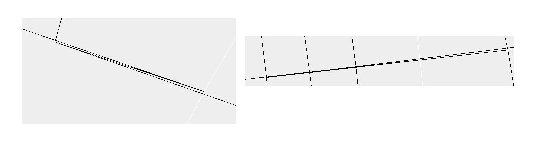
\includegraphics[scale=1.0]{routefailure.eps}
   \caption{Example Failures in Street Map}
   \label{fig:routefailure}
   \end{center}
\end{figure}
\section{Experimental Results}
\label{sec:results}
We repeated the \bmodb{} query execution several times for both data models and
approaches. The tables in Figure \ref{fig:compruntimes} and the graphic in
\ref{fig:CompTotalRunTimesGraphic} compare the average query run times in seconds
for the different scale factors, data models, and approaches.
As you can see, the total run time of all queries in the NDM is around
50\% less than the total query run time of the DMFS at each scale factor.
\begin{figure}[h]
  \begin{minipage}{0.5\linewidth}
    \begin{tiny}
      \begin{tabular}{|c|r|r|r|r|}
        \hline
        &\multicolumn{4}{c|}{\textbf{Scalefactor 0.05}}\\
        \cline{2-5}
        &\multicolumn{2}{c|}{\textbf{DMFS}}&\multicolumn{2}{c|}{\textbf{NDM}}\\
        \hline
        \textbf{Query}&\textbf{OBA}&\textbf{TBA}&\textbf{OBA}&\textbf{TBA}\\
        \hline
        \textbf{1}&0.125&0.109&0.128&0.088\\
        \hline
        \textbf{2}&0.003&0.002&0.003&0.002\\
        \hline
        \textbf{3}&0.245&0.205&0.227&0.268\\
        \hline
        \textbf{4}&6.594&7.514&0.238&0.846\\
        \hline
        \textbf{5}&1.072&1.585&1.098&1.031\\
        \hline
        \textbf{6}&14.332&6.280&3.995&3.675\\
        \hline
        \textbf{7}&3.458&3.191&3.893&3.192\\
        \hline
        \textbf{8}&0.353&0.379&0.201&0.205\\
        \hline
        \textbf{9}&96.724&166.434&19.840&21.783\\
        \hline
        \textbf{10}&104.239&31.555&62.972&76.826\\
        \hline
        \textbf{11}&0.150&0.096&0.224&0.443\\
        \hline
        \textbf{12}&0.296&0.120&0.202&0.226\\
        \hline
        \textbf{13}&9.959&6.551&1.094&1.113\\
        \hline
        \textbf{14}&0.516&0.659&1.566&1.709\\
        \hline
        \textbf{15}&1.144&0.857&0.579&0.488\\
        \hline
        \textbf{16}&6.214&14.354&0.612&1.483\\
        \hline
        \textbf{17}&1.126&0.719&0.228&0.262\\
        \hline
        \textbf{Total}&246.551&240.609&97.061&113.640\\
        \hline
      \end{tabular}
    \end{tiny}
  \end{minipage} \hfill
  \begin{minipage}{0.5\linewidth}
    \begin{tiny}
      \begin{tabular}{|c|r|r|r|r|}
        \hline
        &\multicolumn{4}{c|}{\textbf{Scalefactor 0.2}}\\
        \cline{2-5}
        &\multicolumn{2}{c|}{\textbf{DMFS}}&\multicolumn{2}{c|}{\textbf{NDM}}\\
        \hline
        \textbf{Query}&\textbf{OBA}&\textbf{TBA}&\textbf{OBA}&\textbf{TBA}\\
        \hline
        \textbf{1}&0.123&0.096&0.157&0.099\\
        \hline
        \textbf{2}&0.003&0.003&0.008&0.003\\
        \hline
        \textbf{3}&0.501&0.327&0.424&0.349\\
        \hline
        \textbf{4}&32.323&39.113&0.500&6.522\\
        \hline
        \textbf{5}&1.657&2.985&2.394&2.198\\
        \hline
        \textbf{6}&57.453&45.931&15.508&13.451\\
        \hline
        \textbf{7}&17.184&11.150&27.084&22.814\\
        \hline
        \textbf{8}&0.390&0.379&0.205&0.220\\
        \hline
        \textbf{9}&250.626&386.452&36.323&46.187\\
        \hline
        \textbf{10}&447.679&126.870&286.779&287.101\\
        \hline
        \textbf{11}&0.247&0.165&2.119&2.958\\
        \hline
        \textbf{12}&4.171&0.182&0.262&0.316\\
        \hline
        \textbf{13}&27.028&12.106&5.865&4.669\\
        \hline
        \textbf{14}&1.125&1.143&8.783&9.101\\
        \hline
        \textbf{15}&7.800&3.874&2.543&1.876\\
        \hline
        \textbf{16}&6.441&25.298&0.362&0.776\\
        \hline
        \textbf{17}&8.722&4.042&0.289&0.641\\
        \hline
        \textbf{Total}&863.472&660.217&389,605&399.281\\
        \hline
      \end{tabular}
    \end{tiny}
  \end{minipage}\hfill
\begin{minipage}{0.5\linewidth}
    \begin{tiny}
      \begin{tabular}{|c|r|r|r|r|}
        \hline
        &\multicolumn{4}{c|}{\textbf{Scalefactor 1.0}}\\
        \cline{2-5}
        &\multicolumn{2}{c|}{\textbf{DMFS}}&\multicolumn{2}{c|}{\textbf{NDM}}\\
        \hline
        \textbf{Query}&\textbf{OBA}&\textbf{TBA}&\textbf{OBA}&\textbf{TBA}\\
        \hline
        \textbf{1}&0.196&0.186&0.387&0.185\\
        \hline
        \textbf{2}&0.005&0.004&0.006&0.004\\
        \hline
        \textbf{3}&0.731&0.483&1.020&1.349\\
        \hline
        \textbf{4}&150.172&157.629&2.089&31.769\\
        \hline
         \textbf{5}&3.274&6.079&5.230&5.494\\
        \hline
        \textbf{6}&826.483&2002.002&270.468&235.594\\
        \hline
        \textbf{7}&99.086&53.099&118.840&125.206\\
        \hline
        \textbf{8}&0.794&0.524&0.254&0.398\\
        \hline
        \textbf{9}&775.458&2263.531&106.910&143.150\\
        \hline
        \textbf{10}&3314.518&1942.155&2150.250&1645.812\\
        \hline
        \textbf{11}&0.685&0.474&6.080&7.889\\
        \hline
        \textbf{12}&37.445&0.200&0.272&0.290\\
        \hline
        \textbf{13}&111.587&72.907&26.880&32.540\\
        \hline
        \textbf{14}&11.397&4.238&36.728&37.700\\
        \hline
        \textbf{15}&28.512&16.862&9.696&8.602\\
        \hline
        \textbf{16}&9.726&53.011&0.571&1.880\\
        \hline
        \textbf{17}&86.357&152.542&0.530&6.884\\
        \hline
        \textbf{Total}&5456.427&6725.924&2736.210&2284.747\\
        \hline
      \end{tabular}
    \end{tiny}
  \end{minipage}
 \caption{Compare Query Run Times in Seconds}
 \label{fig:compruntimes}
\end{figure}
\begin{figure}
  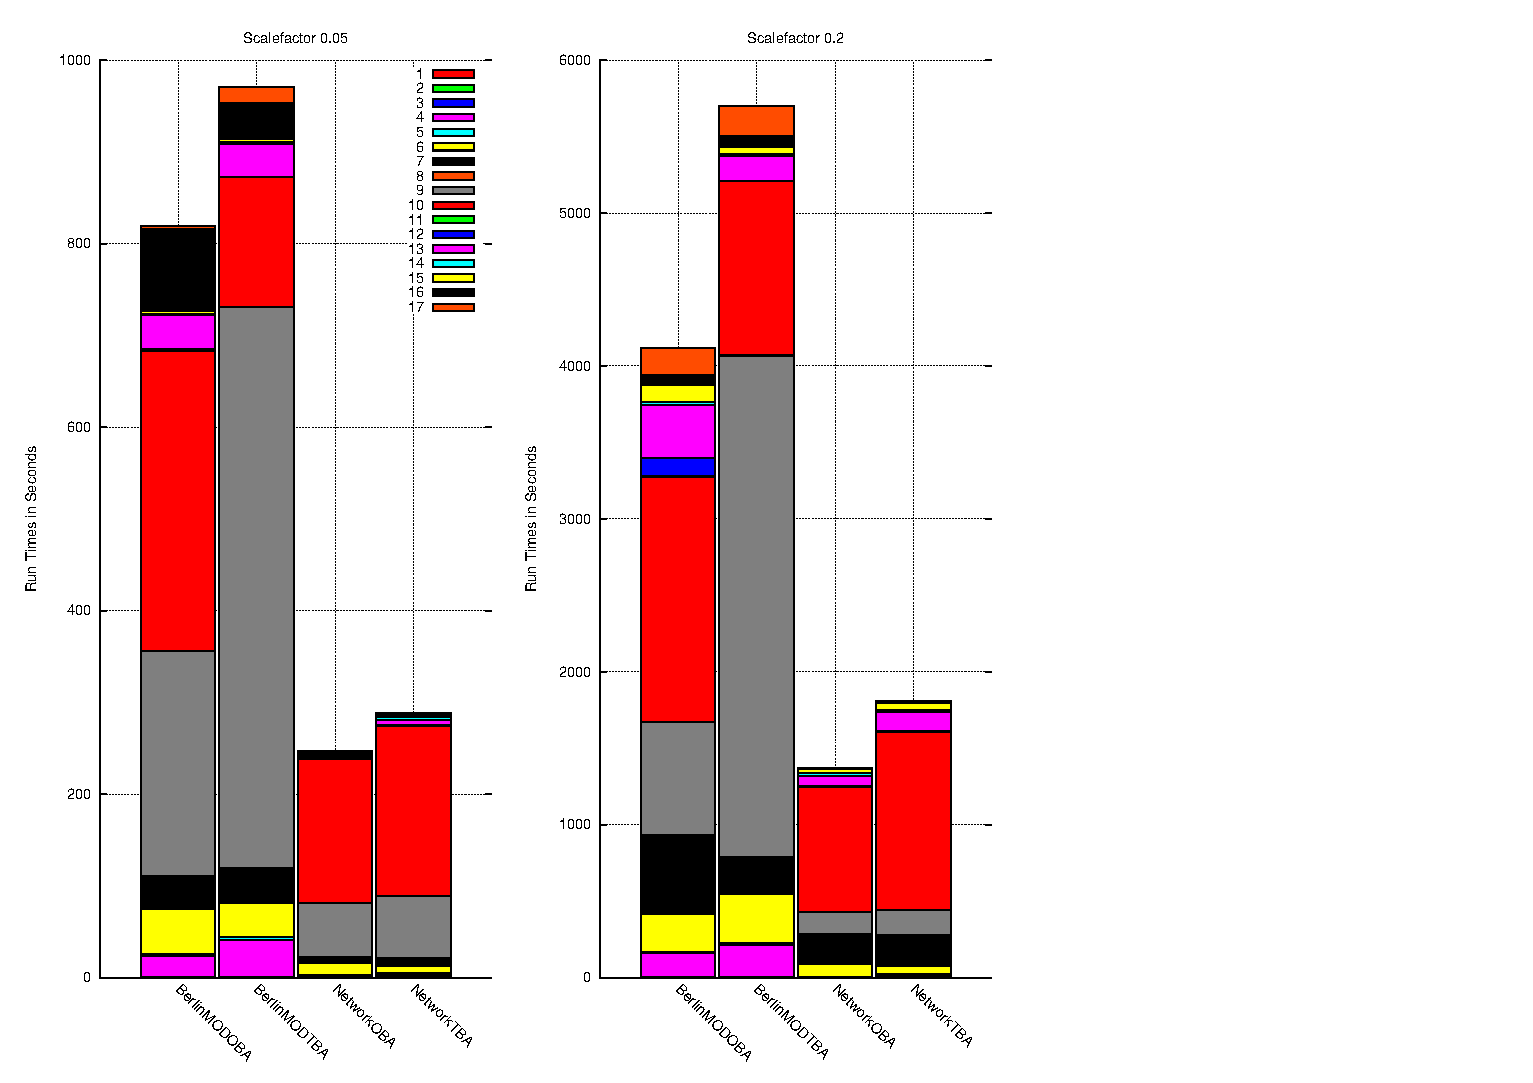
\includegraphics[width=1.0\linewidth]{compruntimesall.eps}
  \caption{Compare Total Run Times}
  \label{fig:CompTotalRunTimesGraphic}
\end{figure}

For the queries 1 and 2, the query run times are almost the same for all data models
and approaches at the different scale factors. This is what we expected because
both queries deal only with standard attributes and standard indexes, which
are not influenced by the different data models.

For query 3, the run times for all data models and approaches are very small. But
we can see a development of the ratio of the run times between the different
data amounts, data models and approaches. Although the query algorithms for both
data models and approaches are almost the same, the run time ratio for the different
amounts of data is different. For the small databases (scale factor 0.05 and 0.2)
the NDM outperforms in the OBA the DMFS, while for scalefactor 1.0 and all TBA
queries the DMFS outperforms the NDM. We think that
two different effects take place. On the one hand, the number of units in the NDM
is less than the number of units in the DMFS,
such that the unit which contains the query time instant can be found faster.
On the other hand, a \dt{gpoint} value has more internal elements (3 \dt{int}, 1 \dt{real},
and 1 \dt{bool}) than a \dt{point} value (2 \dt{real}, and 1 \dt{bool}), such
that result computing and copying is a little more expensive in the NDM.
The advantage of the smaller number of units in a binary search is smaller if
the number of units becomes bigger and the disadvantage of bigger results becomes
greater; that explains the different run time ratios for query 3.

In query 4 the NDM outperforms the DMFS
significantly at all scale factors ($>$ 2 min OBA, $>$ 6 min TBA at scale factor 1.0).
The NDM index used in query 4 is much smaller (OBA 24 MB, TBA 160 MB, at scalefactor 1.0)
than the spatial unit index of the \bmodb{} (OBA 3.7 GB, TBA 3.7 GB at scalefactor 1.0)
and more precise, such that we do not need an additional refinement step after the
index usage in the NDM, like we do in the DMFS.

We expected the NDM to be slower than the DMFS in the queries 5,6, and 10, because
we retranslate intermediate results from the NDM representation into the DMFS representation.
For query 5 this holds in the OBA. We need a little more time in the NDM
than in the DMFS. But in TBA the NDM outperforms the DMFS. This is due to the fact
that a \dt{gline} value has less \dt{RouteInterval}s
than a \dt{line} value representing the same part of a curve has \dt{HalfSegment}s,
such that the union of two or more \dt{gline} values in the aggregate step of query 5 in
TBA can be computed much faster than the union of two or more \dt{line} values.

The NDM outperforms the DMFS again significantly at query 6
for all amounts of data and approaches. In the NDM we reduce the number of candidate
pairs for the distance computation by pre selecting intersecting extended bounding boxes
and use the operation \op{notEverNearerThan} in OBA and TBA, while in the DMFS
in the OBA no filtering is used and the computation is done by
\op{minimum}(\op{distance}($mp1$,$mp2$)$\leq$10.0), and in the TBA the operation
\op{spatialjoin} is used instead of bounding box intersection. While the operation
\op{distance} has always a run time O($n$) the operation \op{everNearerThan}
stops computation immediately if the distance between two units is less than the
query value to reduce computation time. And the operation \op{spatialjoin} of the
\secondo{} DBMS seems to have a big weakness in implementation. Otherwise the
difference in the TBA query run times could not be so big ($>$ 17 min OBA, $>$
80 min TBA, at scale factor 1.0).

After the very good results from query 4 we did not expect query 7 to have such
results in the run times comparison. In fact at scalefactor 1.0 the DMFS outperforms
the NDM significantly in both
approaches and at all scale factors in TBA, while at the smaller scale factors in
OBA the NDM outperforms the DMFS. We think there are two main causes: On the one hand we
have to do the expensive operation \dt{at} for \dt{mgpoint} for the double number
of query \dt{gpoint} compared with the DMFS and
on the other hand the test points out a weakness of the NDM
implementation of the operation \op{at} for \dt{mgpoint}. But in the end, NDM looses
at scale factor 1.0 less than 45 seconds in the OBA respectively less
than 120 seconds in TBA, what is not much compared with the advantages in the
other benchmark queries.

Query 8 is a very fast query in both data models, although the query run time of
the NDM is more than 50\% less than the query run time of the
DMFS. This is caused by the
$length$ attribute of the \dt{mgpoint} and the smaller number of units of a
\dt{mgpoint} compared with the corresponding \dt{mpoint}.

For query 9, the NDM outperforms the DMFS by orders of magnitude. The advantages
named in the analysis of query 8's run time results have a much higher impact
when the number of examined trips becomes bigger. At scale factor 1.0 this saves
more than 10 min time in the OBA and more than 50 min time in the TBA.

The ratio of the run times of query 10 changes between the amounts of data and
both data models. In the OBA and at scale factor 1.0 in the TBA the NDM outperforms
the DMFS at all scale factors, while in the TBA at the two small databases the
DMFS outperforms the NDM significantly. Before our experiments we expected that
the DMFS would outperform the NDM in all cases, because of the expensive
retranslation of intermediate results. So why is the NDM faster ($>$ 20 min in
OBA and $>$ 3 min in TBA at scale factor 1.0) than the DMFS?
In the OBA we use bounding boxes for a preselect of candidate trips that step is not
performed in the DMFS. In the TBA the results are only better for the big amounts
of data we think this is due to the fact that the number of units in \dt{mgpoint}
values is always smaller than in \dt{mpoint} values such that the final aggregation
of the different trips of the same cars can be done faster in the NDM
than in the DMFS.

Query 11 is identical with the first part of query 12. So it is surprising that
the run time of query 11 at scalefactor 1.0 is longer than the run time of query 12,
which does additional computations. In our experiments with the different queries
we have seen that there exist numerous cache effects depending on the sequence of
the queries. So we think that query 12 takes profit cache effects resulting from
query 11 running immediately before query 12. Another weakness of the NDM pointed
out by the run times of query 11 and query 14 is that our
network-temporal position index has bad run times for query $netbox$ objects
constructed from a single \dt{gpoint} and a single time instant. This becomes worse
with a higher number of indexed units. As you can see at query 15 this does not
hold for query $netboxes$ constructed from a single \dt{gpoint} and a time interval.
We have to spend some more work to figure out the problem and develop a better
network-temporal position index to improve our NDM system.

In our experiments we also tested the MON-Tree \cite{MONTreeAlmeidaGeoinformatica} as network-temporal
index but the elapsed run time performance was not good, although the CPU run times
was were small.

The bad performance of the network-temporal position index is also shown by query 13.
The NDM outperforms the DMFS significantly, but we do not use any index in the
executable NDM queries, while the DMFS uses its spatio-temporal index to preselect
candidate trips. The same holds for query 17.

The NDM version of query 16 takes profit from the smaller number
of units in the NDM and outperforms the data model of free movement
in two dimensional space.

Although we detected in our experiments some points of weakness in the network-temporal
position indexing, the NDM outperforms the DMFS by orders of magnitude. The weakness
of the NDM mostly occurs in queries with short run times, whereas the advantages
of the NDM become apparent in the queries with long run times, such that the weakness
of the network-temporal position index is covered by the advantages of the network
data model.
\section{Summary and Future Work}
\label{sec:summary}
We presented our translation of the \bmodb{} into the NDM and
compared the capabilities of both data models, with very good results for the
NDM. Our experiments show that the NDM outperforms
the DMFS by orders of magnitude with respect to storage space and query run times.
This is mainly caused by the much lower number of units for an \dt{mgpoint} value
compared with the number of units of the corresponding \dt{mpoint}, which also
results in smaller indexes for the NDM objects. The \bmodb{} of the NDM pointed out
that we should spend time in the improvement of the network-temporal position index
and the \op{at} operation for \dt{mgpoint} and \dt{gpoint} values.

The good results of the NDM encourage us to work on an extension
of the \bmodb{}, which should enable us to compare the capabilities of different
spatio-temporal NDMs with respect to the special challenges of
NDM, like shortest path and fastest path computation.

Another direction of our actual work is traffic flow estimation and traffic jam
representation in the NDM.

Another interesting topic for future work on the NDMs is the efficient
computation of dynamic network distances between moving network objects.
\bibliography{BerlinMODAndNetworkDataModel}{}
\bibliographystyle{plain}
\end{document}
